% https://github.com/josephwright/beamer/blob/main/doc/solutions/generic-talks/generic-ornate-15min-45min.en.tex
\documentclass[aspectratio=169]{beamer}

\definecolor{confirm-gray}{RGB}{126, 126, 126}

\mode<presentation>
{
    \usetheme{Madrid}
    \usecolortheme{default}
    \setbeamercovered{transparent}
}

\setbeamertemplate{navigation symbols}{}
\setbeamersize{text margin left=25pt, text margin right=25pt}

\usepackage{appendixnumberbeamer}
\usepackage[czech]{babel}
\usepackage[export]{adjustbox}
\usepackage{ragged2e}

\title{Systém pro sportovní kluby}
\author{Lukáš Paukert}

\institute[]{\\
    \vspace{-10pt}
    Vedoucí práce: Ing. Filip Glazar\\
    \vspace{15pt}
    Fakulta informačních technologií\\
    České vysoké učení technické v Praze
}

\titlegraphic{
\includegraphics[width=1.5cm]{images/ctu-logo.pdf}}

% If you have a file called "university-logo-filename.xxx", where xxx
% is a graphic format that can be processed by latex or pdflatex,
% resp., then you can add a logo as follows:

% \pgfdeclareimage[height=0.5cm]{university-logo}{university-logo-filename}
% \logo{\pgfuseimage{university-logo}}


% If you wish to uncover everything in a step-wise fashion, uncomment
% the following command: 

%\beamerdefaultoverlayspecification{<+->}

\begin{document}

\begin{frame}
    \titlepage
\end{frame}

\begin{frame}{Motivace}
    \begin{figure}
        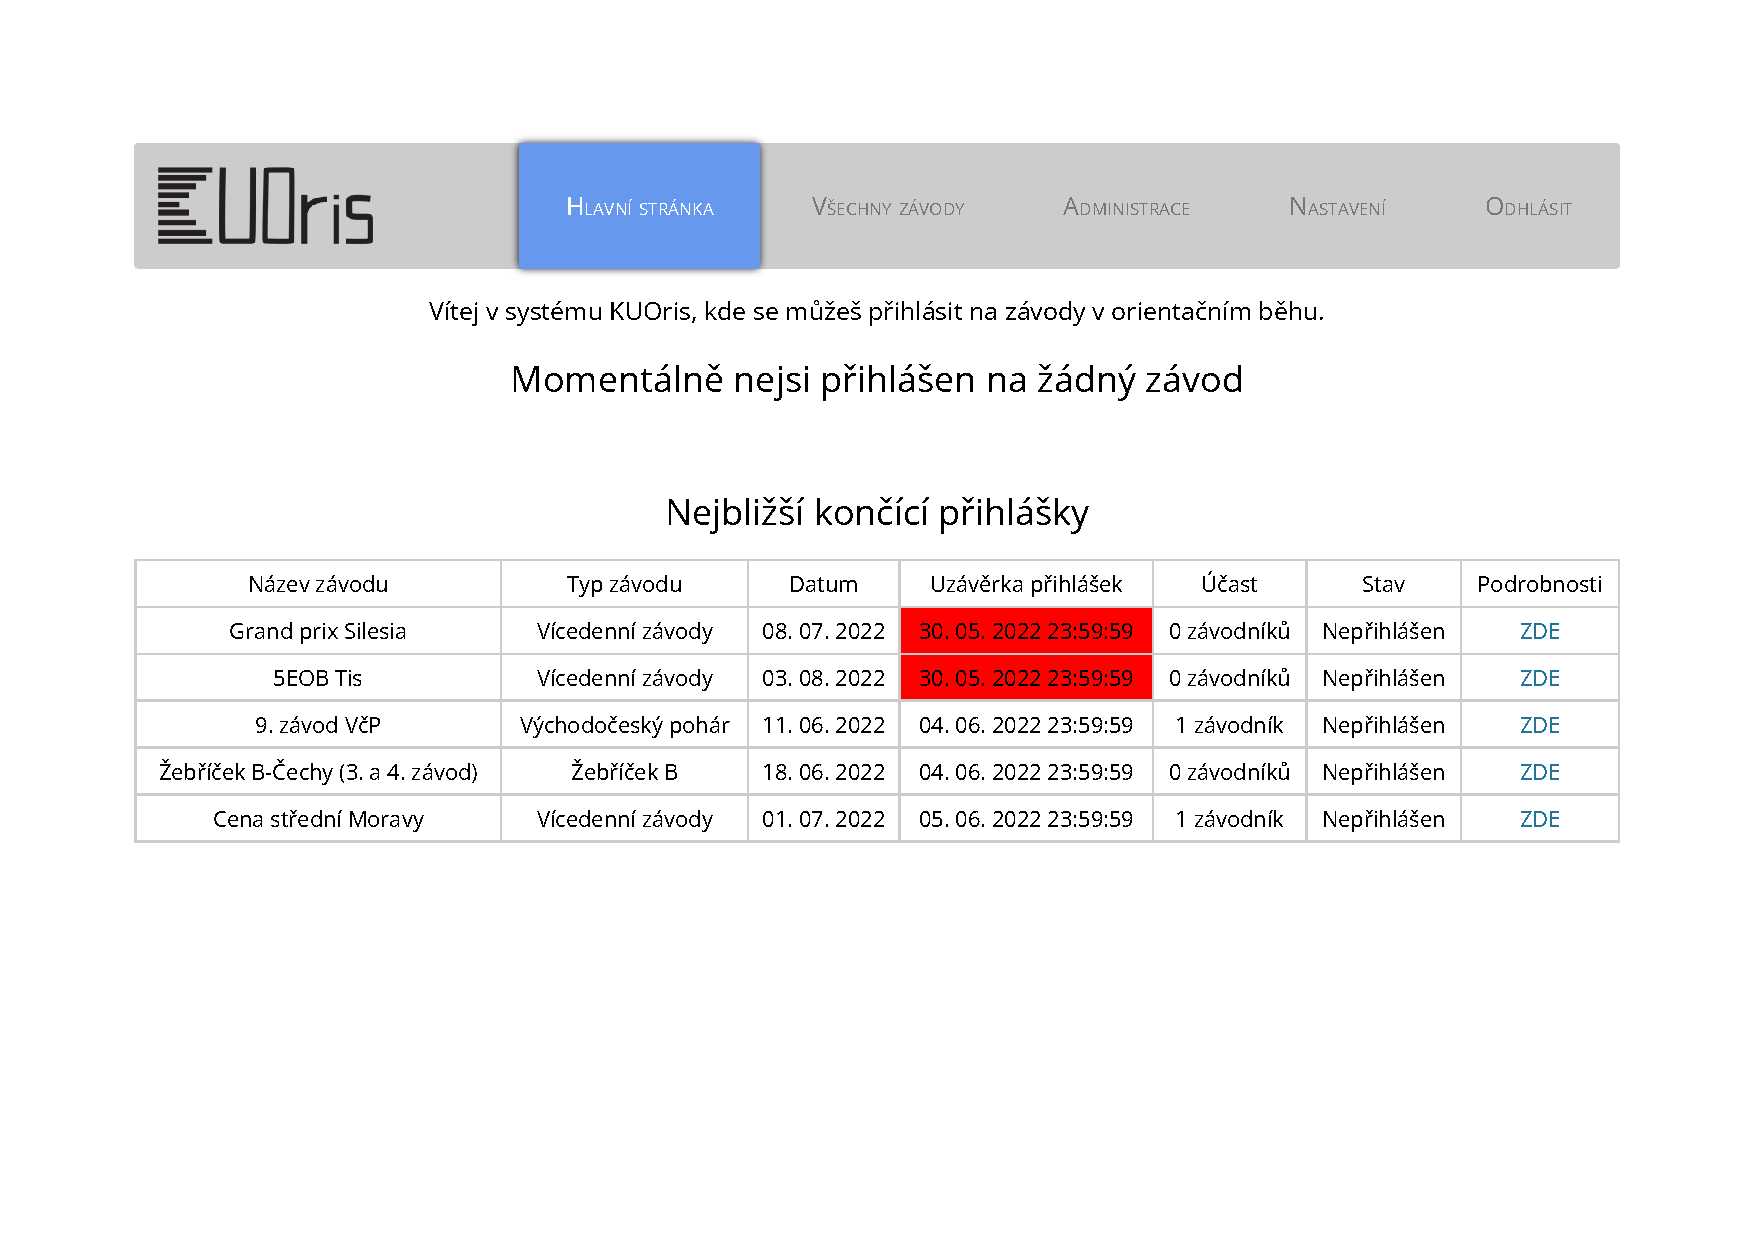
\includegraphics[width=0.9\linewidth, cfbox=lightgray 0.5pt 5pt]{images/kuoris.pdf}
    \end{figure}
\end{frame}

\begin{frame}{Zadání}
    \begin{itemize}
        \item vytvoření webové aplikace pro sportovní kluby
        \item evidence a správa uživatelů a událostí
        \item propojení s informačním systémem ORIS
        \item postup: analýza, návrh, implementace, uživatelské testování, příprava na nasazení 
    \end{itemize}
\end{frame}

\begin{frame}{Technologie}
    \begin{itemize}
        \item výběr podřízen aktuálně využívaným hostingovým službám
        \item zvolené technologie
        \begin{itemize}
            \item PHP
            \item Symfony
            \item MariaDB
            \item Bootstrap
        \end{itemize}
    \end{itemize}
\end{frame}

\begin{frame}{Implementace}{ORIS API}
    \begin{itemize}
        \item komunikace pomocí \texttt{GET} požadavků s minimálně 2 query parametry
        \begin{itemize}
            \item \texttt{format}
            \item \texttt{method}
        \end{itemize}
        \item v současné době je podporováno 28 různých metod
        \item vytvořená aplikace využívá 3 metody
        \begin{itemize}
            \item \texttt{getEvent}
            \item \texttt{getEventList}
            \item \texttt{createEntry}
        \end{itemize}
    \end{itemize}
\end{frame}

\begin{frame}{Implementace}{Formuláře}
    \begin{figure}
        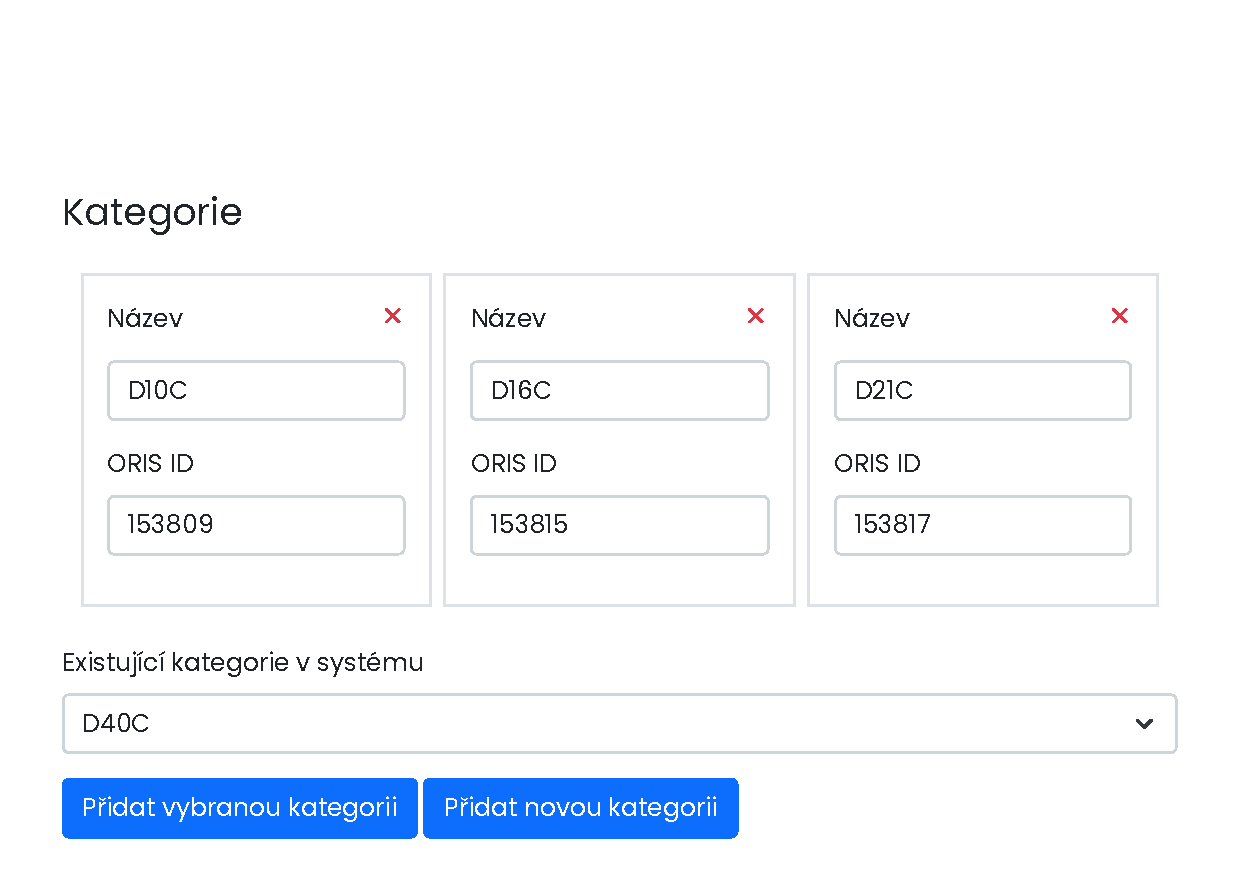
\includegraphics[width=0.65\linewidth, cfbox=lightgray 0.5pt 10pt]{images/categories.pdf}
    \end{figure}
\end{frame}

\begin{frame}{Implementace}{Responzivní design}
    \begin{figure}[h]
        \hfill
        \begin{minipage}[b]{0.3\linewidth}
            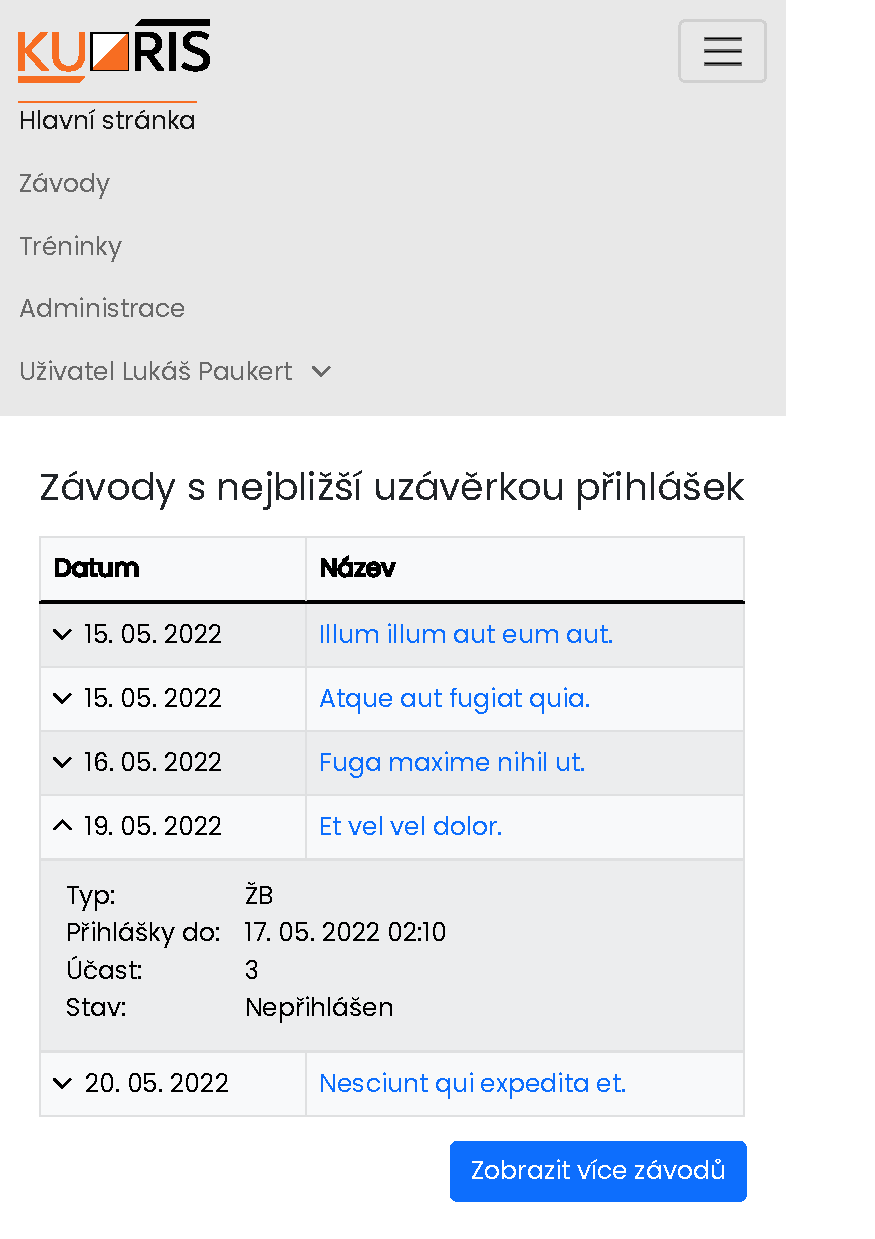
\includegraphics[width=0.9\linewidth, cfbox=lightgray 0.5pt 0pt]{images/homepage.pdf}
        \end{minipage}
        \hfill
        \begin{minipage}[b]{0.3\linewidth}
            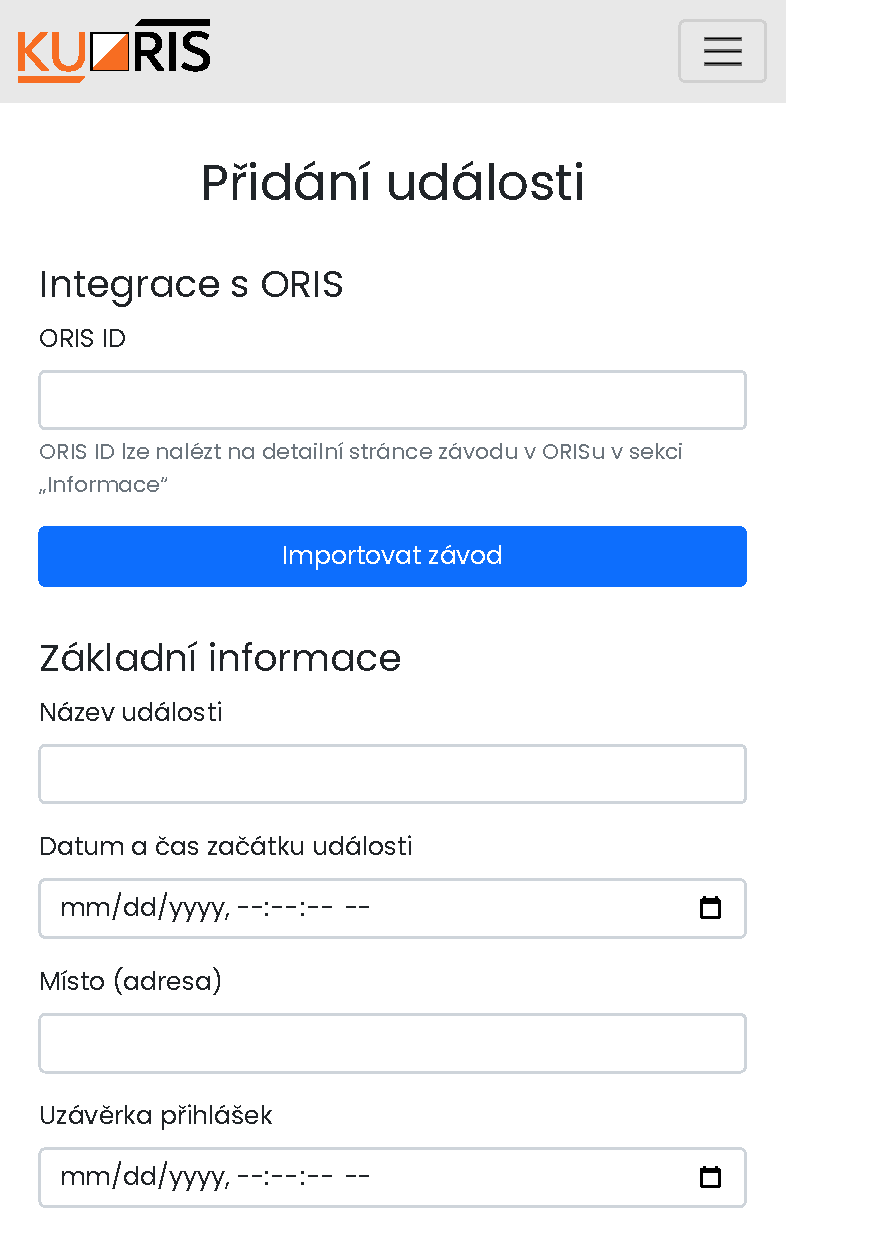
\includegraphics[width=0.9\linewidth, cfbox=lightgray 0.5pt 0pt]{images/add-race.pdf}
        \end{minipage}
        \hfill
        \begin{minipage}[b]{0.3\linewidth}
            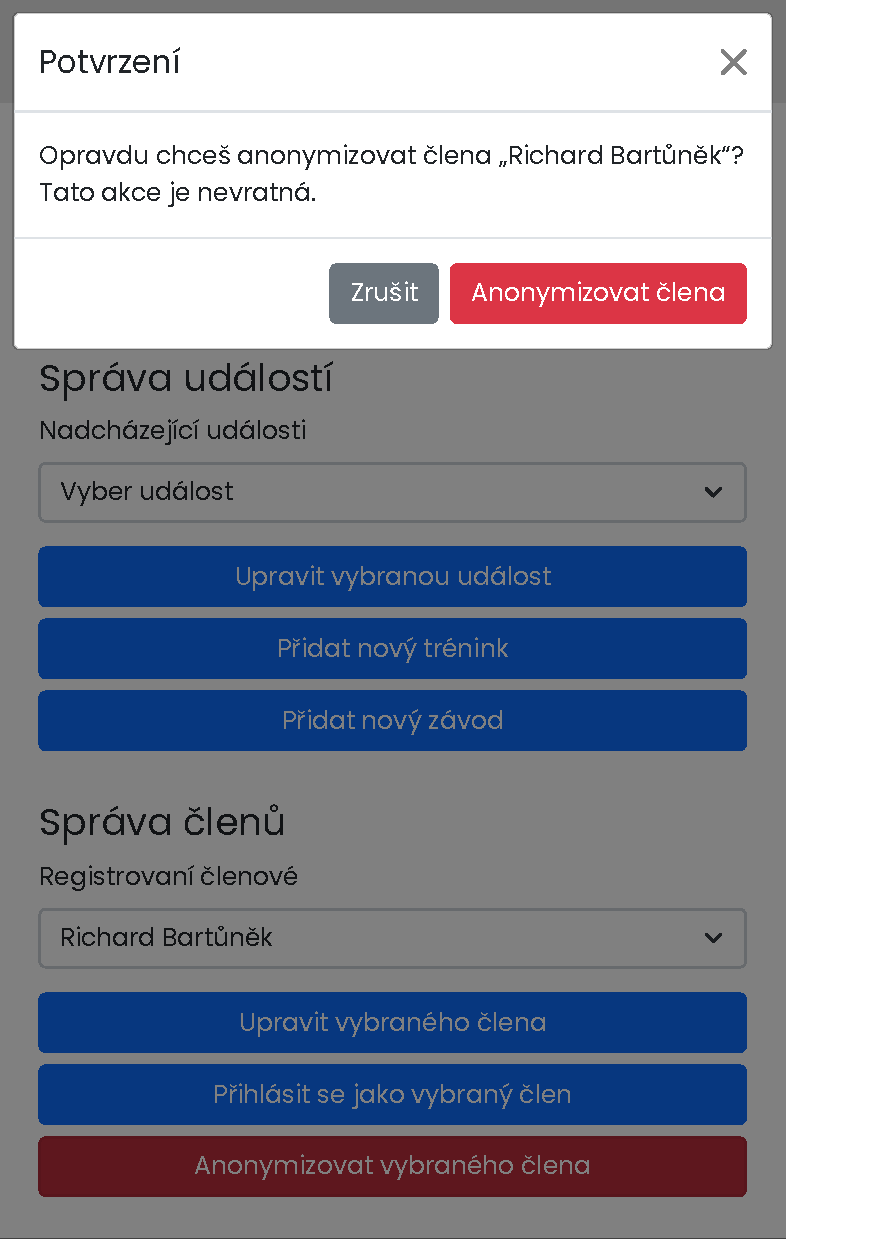
\includegraphics[width=0.9\linewidth, cfbox=confirm-gray 0.5pt 0pt]{images/confirm-dialog.pdf}
        \end{minipage}
        \hfill
    \end{figure}
\end{frame}

\begin{frame}{Závěr}
    \begin{itemize}
        \item všechny cíle práce byly splněny
        \item aplikace je připravena pro nasazení
        \item možná vylepšení
        \begin{itemize}
            \item e-mailové notifikace při přidání nové události
            \item pokročilejší propojení s informačním systémem ORIS
            \item zobrazování statistik pro trenéry a administrátory
        \end{itemize}
    \end{itemize}
\end{frame}

\begin{frame}
    \centering
    \vspace{10pt}
    \Huge Děkuji za pozornost
\end{frame}

\appendix

\begin{frame}{Otázky k obhajobě}{Oponent práce: Ing. Oldřich Malec}
    \begin{itemize}
        \justifying
        \item Jeden z nefunkčních požadavků je pevně zvolená technologie kvůli hostingu. V textu pak dokonce i popisujete obtíže s nasazením na zvolený hosting. Zkoušel jste, ze své pozice softwarového inženýra, diskutovat se zadavatelem (či plátcem hostingu), že toto není v dnešní době ideální řešení, a alternativy existují?
        \vspace{10pt}
        \item V ORIS API jste našel obří bezpečnostní mezeru. Jak jste na ni, kromě komentáře ve~svém textu, reagoval? Zkoušel jste např. kontaktovat vývojáře ORIS API, aby toto opravili?
    \end{itemize}
\end{frame}

\end{document}
